
\documentclass[letterpaper,hide notes,xcolor={table,svgnames},pdftex]{beamer}
\def\showexamples{t}


%\usepackage[svgnames]{xcolor}

%% Demo talk
%\documentclass[letterpaper,notes=show]{beamer}

\usecolortheme{crane}%seahorse crane
\setbeamertemplate{navigation symbols}{}

\usetheme{MyPittsburgh}
%\usetheme{Frankfurt}

%\usepackage{tipa}

\usepackage{hyperref}
\usepackage{graphicx,xspace}
\usepackage[normalem]{ulem}

\newcommand\SF[1]{$\bigstar$\footnote{SF: #1}}

\usepackage{paratype}
\renewcommand*\familydefault{\sfdefault} %% Only if the base font of the document is to be sans serif
\usepackage[zerostyle=c]{newtxtt}
\usepackage[T1]{fontenc}

\newcounter{tmpnumSlide}
\newcounter{tmpnumNote}

\usepackage{xcolor}
\usepackage{tabu}
\definecolor{light-gray}{gray}{0.75}
\taburulecolor{light-gray}

% old question code
%\newcommand\question[1]{{$\bigstar$ \small \onlySlide{2}{#1}}}
% \newcommand\nquestion[1]{\ifdefined \presentationonly \textcircled{?} \fi \note{\par{\Large \textbf{?}} #1}}
% \newcommand\nanswer[1]{\note{\par{\Large \textbf{A}} #1}}


 \newcommand\mnote[1]{%
   \addtocounter{tmpnumSlide}{1}
   \ifdefined\showcues {~\tiny\fbox{\arabic{tmpnumSlide}}}\fi
   \note{\setlength{\parskip}{1ex}\addtocounter{tmpnumNote}{1}\textbf{\Large \arabic{tmpnumNote}:} {#1\par}}}

\newcommand\mmnote[1]{\note{\setlength{\parskip}{1ex}#1\par}}

%\newcommand\mnote[2][]{\ifdefined\handoutwithnotes {~\tiny\fbox{#1}}\fi
% \note{\setlength{\parskip}{1ex}\textbf{\Large #1:} #2\par}}

%\newcommand\mnote[2][]{{\tiny\fbox{#1}} \note{\setlength{\parskip}{1ex}\textbf{\Large #1:} #2\par}}

\newcommand\mquestion[2]{{~\color{red}\fbox{?}}\note{\setlength{\parskip}{1ex}\par{\Large \textbf{?}} #1} \note{\setlength{\parskip}{1ex}\par{\Large \textbf{A}} #2\par}\ifdefined \presentationonly \pause \fi}

\newcommand\blackboard[1]{%
\ifdefined   \showblackboard
  {#1}
  \else {\begin{center} \fbox{\colorbox{blue!30}{%
         \begin{minipage}{.95\linewidth}%
           \hspace{\stretch{1}} Some space intentionally left blank; done at the blackboard.%
         \end{minipage}}}\end{center}}%
         \fi%
}



%\newcommand\q{\tikz \node[thick,color=black,shape=circle]{?};}
%\newcommand\q{\ifdefined \presentationonly \textcircled{?} \fi}

\usepackage{listings}
\lstset{%
  keywordstyle=\bfseries,
  aboveskip=15pt,
  belowskip=15pt,
  captionpos=b,
  identifierstyle=\ttfamily,
  escapeinside={(*@}{@*)},
  stringstyle=\ttfamiliy,
  frame=lines,
  numbers=left, basicstyle=\scriptsize, numberstyle=\tiny, stepnumber=0, numbersep=2pt}

\usepackage{siunitx}
\newcommand\sius[1]{\num[group-separator = {,}]{#1}\si{\micro\second}}
\newcommand\sims[1]{\num[group-separator = {,}]{#1}\si{\milli\second}}
\newcommand\sins[1]{\num[group-separator = {,}]{#1}\si{\nano\second}}
\sisetup{group-separator = {,}, group-digits = true}

%% -------------------- tikz --------------------
\usepackage{tikz}
\usetikzlibrary{positioning}
\usetikzlibrary{arrows,backgrounds,automata,decorations.shapes,decorations.pathmorphing,decorations.markings,decorations.text}

\tikzstyle{place}=[circle,draw=blue!50,fill=blue!20,thick, inner sep=0pt,minimum size=6mm]
\tikzstyle{transition}=[rectangle,draw=black!50,fill=black!20,thick, inner sep=0pt,minimum size=4mm]

\tikzstyle{block}=[rectangle,draw=black, thick, inner sep=5pt]
\tikzstyle{bullet}=[circle,draw=black, fill=black, thin, inner sep=2pt]

\tikzstyle{pre}=[<-,shorten <=1pt,>=stealth',semithick]
\tikzstyle{post}=[->,shorten >=1pt,>=stealth',semithick]
\tikzstyle{bi}=[<->,shorten >=1pt,shorten <=1pt, >=stealth',semithick]

\tikzstyle{mut}=[-,>=stealth',semithick]

\tikzstyle{treereset}=[dashed,->, shorten >=1pt,>=stealth',thin]

\usepackage{ifmtarg}
\usepackage{xifthen}
\makeatletter
% new counter to now which frame it is within the sequence
\newcounter{multiframecounter}
% initialize buffer for previously used frame title
\gdef\lastframetitle{\textit{undefined}}
% new environment for a multi-frame
\newenvironment{multiframe}[1][]{%
\ifthenelse{\isempty{#1}}{%
% if no frame title was set via optional parameter,
% only increase sequence counter by 1
\addtocounter{multiframecounter}{1}%
}{%
% new frame title has been provided, thus
% reset sequence counter to 1 and buffer frame title for later use
\setcounter{multiframecounter}{1}%
\gdef\lastframetitle{#1}%
}%
% start conventional frame environment and
% automatically set frame title followed by sequence counter
\begin{frame}%
\frametitle{\lastframetitle~{\normalfont(\arabic{multiframecounter})}}%
}{%
\end{frame}%
}
\makeatother

\makeatletter
\newdimen\tu@tmpa%
\newdimen\ydiffl%
\newdimen\xdiffl%
\newcommand\ydiff[2]{%
    \coordinate (tmpnamea) at (#1);%
    \coordinate (tmpnameb) at (#2);%
    \pgfextracty{\tu@tmpa}{\pgfpointanchor{tmpnamea}{center}}%
    \pgfextracty{\ydiffl}{\pgfpointanchor{tmpnameb}{center}}%
    \advance\ydiffl by -\tu@tmpa%
}
\newcommand\xdiff[2]{%
    \coordinate (tmpnamea) at (#1);%
    \coordinate (tmpnameb) at (#2);%
    \pgfextractx{\tu@tmpa}{\pgfpointanchor{tmpnamea}{center}}%
    \pgfextractx{\xdiffl}{\pgfpointanchor{tmpnameb}{center}}%
    \advance\xdiffl by -\tu@tmpa%
}
\makeatother
\newcommand{\copyrightbox}[3][r]{%
\begin{tikzpicture}%
\node[inner sep=0pt,minimum size=2em](ciimage){#2};
\usefont{OT1}{phv}{n}{n}\fontsize{4}{4}\selectfont
\ydiff{ciimage.south}{ciimage.north}
\xdiff{ciimage.west}{ciimage.east}
\ifthenelse{\equal{#1}{r}}{%
\node[inner sep=0pt,right=1ex of ciimage.south east,anchor=north west,rotate=90]%
{\raggedleft\color{black!50}\parbox{\the\ydiffl}{\raggedright{}#3}};%
}{%
\ifthenelse{\equal{#1}{l}}{%
\node[inner sep=0pt,right=1ex of ciimage.south west,anchor=south west,rotate=90]%
{\raggedleft\color{black!50}\parbox{\the\ydiffl}{\raggedright{}#3}};%
}{%
\node[inner sep=0pt,below=1ex of ciimage.south west,anchor=north west]%
{\raggedleft\color{black!50}\parbox{\the\xdiffl}{\raggedright{}#3}};%
}
}
\end{tikzpicture}
}


%% --------------------

%\usepackage[excludeor]{everyhook}
%\PushPreHook{par}{\setbox0=\lastbox\llap{MUH}}\box0}

%\vspace*{\stretch{1}

%\setbox0=\lastbox \llap{\textbullet\enskip}\box0}

\setlength{\parskip}{\fill}

\newcommand\noskips{\setlength{\parskip}{1ex}}
\newcommand\doskips{\setlength{\parskip}{\fill}}

\newcommand\xx{\par\vspace*{\stretch{1}}\par}
\newcommand\xxs{\par\vspace*{2ex}\par}
\newcommand\tuple[1]{\langle #1 \rangle}
\newcommand\code[1]{{\sf \footnotesize #1}}
\newcommand\ex[1]{\uline{Example:} \ifdefined \presentationonly \pause \fi
  \ifdefined\showexamples#1\xspace\else{\uline{\hspace*{2cm}}}\fi}

\newcommand\ceil[1]{\lceil #1 \rceil}


\AtBeginSection[]
{
   \begin{frame}
       \frametitle{Outline}
       \tableofcontents[currentsection]
   \end{frame}
}



\pgfdeclarelayer{edgelayer}
\pgfdeclarelayer{nodelayer}
\pgfsetlayers{edgelayer,nodelayer,main}

\tikzstyle{none}=[inner sep=0pt]
\tikzstyle{rn}=[circle,fill=Red,draw=Black,line width=0.8 pt]
\tikzstyle{gn}=[circle,fill=Lime,draw=Black,line width=0.8 pt]
\tikzstyle{yn}=[circle,fill=Yellow,draw=Black,line width=0.8 pt]
\tikzstyle{empty}=[circle,fill=White,draw=Black]
\tikzstyle{bw} = [rectangle, draw, fill=blue!20, 
    text width=4em, text centered, rounded corners, minimum height=2em]
    
    \newcommand{\CcNote}[1]{% longname
	This work is licensed under the \textit{Creative Commons #1 3.0 License}.%
}
\newcommand{\CcImageBy}[1]{%
	\includegraphics[scale=#1]{creative_commons/cc_by_30.pdf}%
}
\newcommand{\CcImageSa}[1]{%
	\includegraphics[scale=#1]{creative_commons/cc_sa_30.pdf}%
}
\newcommand{\CcImageNc}[1]{%
	\includegraphics[scale=#1]{creative_commons/cc_nc_30.pdf}%
}
\newcommand{\CcGroupBySa}[2]{% zoom, gap
	\CcImageBy{#1}\hspace*{#2}\CcImageNc{#1}\hspace*{#2}\CcImageSa{#1}%
}
\newcommand{\CcLongnameByNcSa}{Attribution-NonCommercial-ShareAlike}


\newenvironment{changemargin}[1]{% 
  \begin{list}{}{% 
    \setlength{\topsep}{0pt}% 
    \setlength{\leftmargin}{#1}% 
    \setlength{\rightmargin}{1em}
    \setlength{\listparindent}{\parindent}% 
    \setlength{\itemindent}{\parindent}% 
    \setlength{\parsep}{\parskip}% 
  }% 
  \item[]}{\end{list}} 




\title{Lecture 1 --- Introduction to the Course}

\author{J. Zarnett\\
\texttt{jzarnett@uwaterloo.ca}}
\institute{Department of Electrical and Computer Engineering \\
  University of Waterloo}
\date{\today}

\begin{document}

\begin{frame}
  \titlepage
  
  \begin{center}
  \small{Acknowledgments: W.D. Bishop}
  \end{center}
 \end{frame}
 
\begin{frame}
\frametitle{Course Objectives}

\textit{The purpose of computing is insight, not numbers.}\\
\hfill - R. W. Hamming

Goal: students gain insight into software design \& construction.

You will have an opportunity to achieve the following three goals:
\begin{enumerate}
\item Learn to develop algorithms to solve programming problems
\item Acquire an understanding of a programming language
\item Establish a foundation for future courses
\end{enumerate}

\end{frame}

\begin{frame}
\frametitle{Course Syllabus}
As our first order of business, we'll go over the course syllabus.
\end{frame}

\begin{frame}
\frametitle{What is a Computer?}

\alert{Computer}: a programmable device that can store, retrieve, and process data.

\alert{Program}: to work out a sequence of operations to be performed by a mechanism.

(Merriam-Webster Online Dictionary Definitions)

\end{frame}


\begin{frame}
\frametitle{Definition of a Computer}

The formal definition of a computer system encompasses devices other than just personal computers.

Embedded computer systems use computing devices to control other systems:

\begin{itemize}
\item Anti-lock braking systems
\item MP3 players
\item Cellular phones
\item Televisions
\end{itemize}

Statistically speaking, personal computers (PCs) represent a very small fraction of the computer marketplace.

\end{frame}

\begin{frame}
\frametitle{History of the Programmable Computer}
\underline{Z3 (1941)}\\
\quad Lacked support for conditional branch instructions

\underline{Colossus (1943)}\\
\quad Targeted a specific application (code breaking)

\underline{Harvard Mark I (1944)}\\
\quad Used separate storage units for instructions \& data

\underline{ENIAC (1946)}\\
\quad Required hard-wiring of the control paths.

\underline{Manchester Baby (1948)}\\
\quad Implemented first working von Neumann computer architecture.

\end{frame}

\begin{frame}
\frametitle{About the ENIAC}

Built in 1944, the ENIAC had the following components:
\begin{itemize}
	\item 17 468 vacuum tubes
	\item 1 500 relays
	\item 7 200 crystal diodes
	\item 70 000 resistors
	\item 10 000 capacitors
	\item 5 000 000 hand-soldered joints
\end{itemize}

\end{frame}

\begin{frame}
\frametitle{About the ENIAC}

The ENIAC had the following properties:
\begin{itemize}
	\item 30 tons in weight
	\item 167 m$^{3}$ in volume
	\item 160 kW of power consumption
\end{itemize}

\end{frame}

\begin{frame}
\frametitle{ENIAC}
\begin{center}
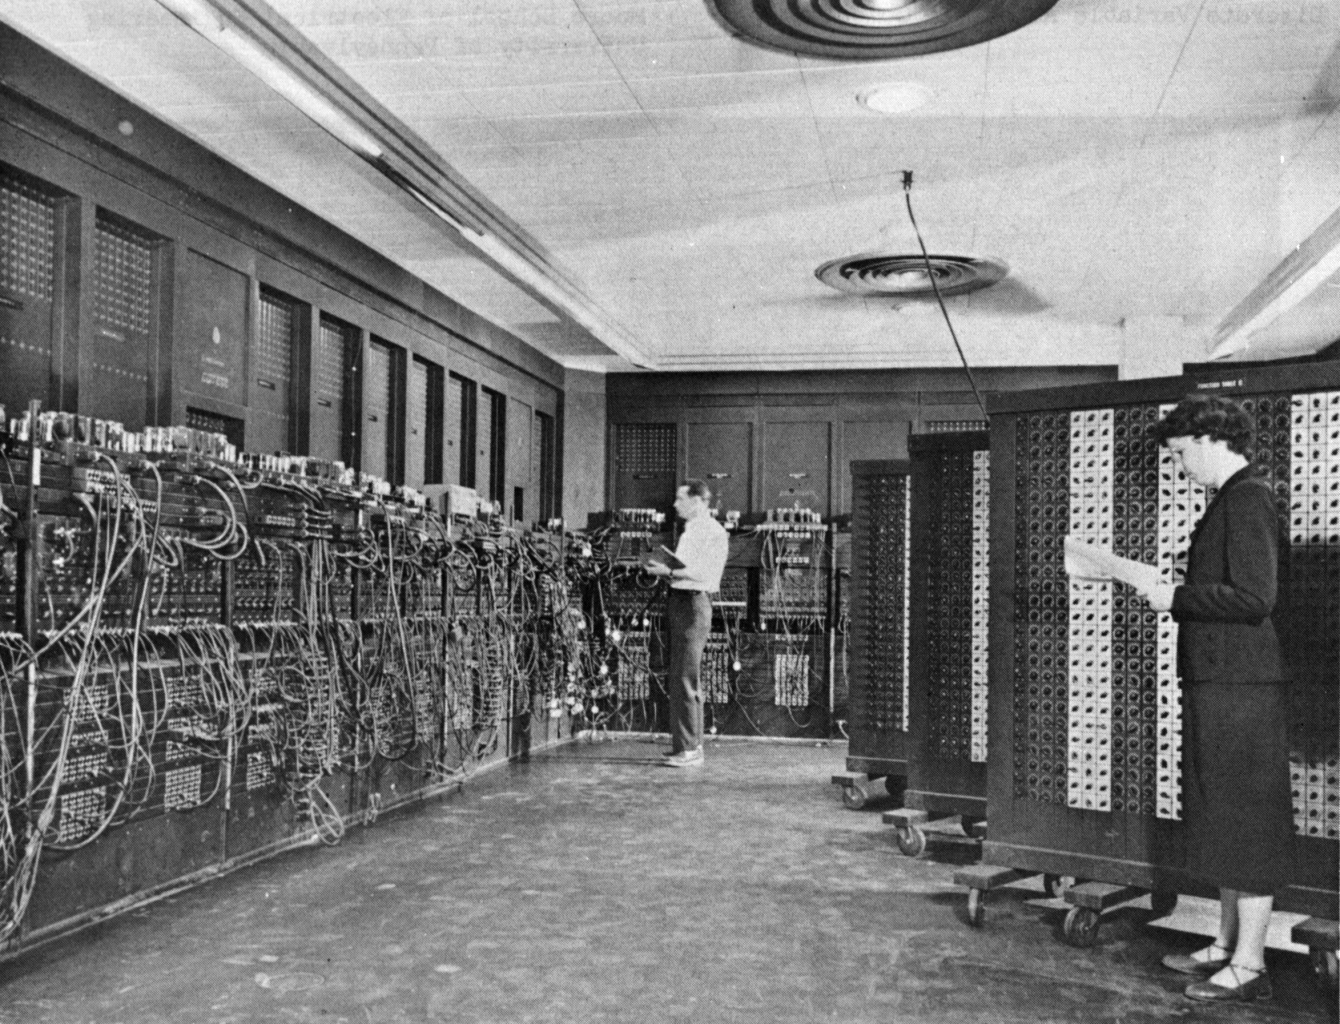
\includegraphics[width=0.75\textwidth]{images/eniac.jpg}

\tiny{Source: \texttt{http://en.wikipedia.org/wiki/ENIAC}}
\end{center}


\end{frame}

\begin{frame}
\frametitle{Computer Development Milestones}
{\tiny
\begin{center}
\begin{tabular}{|p{1cm}|p{2cm}|p{3cm}|p{3.5cm}|}
	\hline
	\textbf{Generation} & \textbf{Technology} & \textbf{Examples} & \textbf{Comments}\\ \hline 
	$0^{th}$ \mbox{(1642-1940)} & Mechanical Systems & Pascalene, Analytical Engine & Simple machines performing addition and subtraction \\\hline
	$1^{st}$ \mbox{(1940-1955)} & Vacuum Tubes & Z3, Colussus, ENIAC, EDVAC, Harvard Mark I, IBM 701, Manchester Baby, Univac I & Mostly special purpose computers for military applications \\\hline
	$2^{nd}$ \mbox{(1955-1965)} & Transistors & DEC PDP-1, IBM 7030, CDC 6600 & Computers with support for high level programming languages \\\hline
	$3^{rd}$ \mbox{(1965-1975)} & Integrated Circuits & DEC PDP-8, DEC PDP-11, IBM System/360 & Computers with faster memory and operating systems \\\hline
	$4^{th}$ \mbox{(1975-1990)} & Very Large Scale Integration (VLSI) & DEC MicroVAX, IBM 3090, IBM PC, Cray X-MP, Osborne 1, Apple II, Apple Macintosh & First personal computers and the first portable computers \\\hline
	$5^{th}$ \mbox{(1990-)} & Nanotechnology, Massive Parellelism & IBM BlueGene/L, IBM x345, OLPC, Apple Macbook, Sun Ultra II & Massive supercomputers, powerful workstations, portable computers \\\hline
	
\end{tabular}

\tiny{Source: IEEE Computer Society (http://www.computer.org/portal/cms\_docs\_computer/computer/timeline/timeline.pdf)}

\end{center}
}

\end{frame}

\begin{frame}
\frametitle{Digital Computers}
A \alert{Digital Computer} uses electronic circuits to implement a programmable computer.

All information within a digital computer is represented using a sequence of \texttt{0}s and \texttt{1}s.

Typically built using chips known as ASICs (Application-Specific Integrated Circuits) made of millions of transistors.

\end{frame}

\begin{frame}
\frametitle{von Neumann Computer Architecture}

\begin{center}
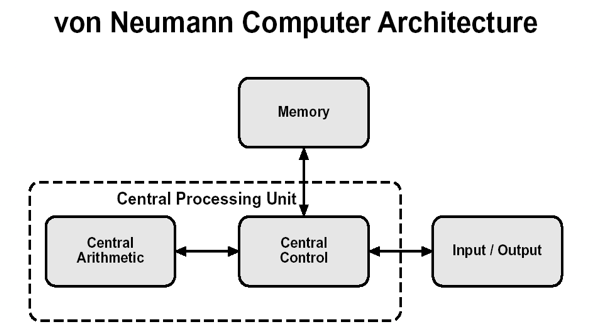
\includegraphics[width=0.75\textwidth]{images/vonNeumann.png}
\end{center}

\tiny{Source: J. von Neumann, First Draft of a Report on the EDVAC.  Technical Report W-6700RD-492, Moore School of Electrical Engineering, University of Pennsylvania, June 1945.}

\end{frame}

\begin{frame}
\frametitle{Software Construction Fundamentals}
Before learning to program, let's examine why people program...

Computers are best suited to solving problems that involve repetitive processing or large amounts of data.

Computers do not (yet) exhibit intelligence like humans.

They do exactly what they are instructed to do.

\end{frame}


\begin{frame}
\frametitle{Why Create Software?}
Computers are well-suited to reliably performing repetitive tasks.

Humans get distracted and this leads to mistakes.

Computers don't get bored!

Also, computers are often much faster...

\end{frame}

\begin{frame}
\frametitle{Why Create Software?}

Imagine your task is to calculate the sum of integers from 1 to 10 000.

You can do this with a calculator, but: slow, boring, error-prone.

\end{frame}

\begin{frame}
\frametitle{Summing Integers: Analytical Approach}

A smart student might observe that half the values will be 5,000 or less and half the values will be 5,001 or more. 

Estimate the result to be close to 50,000,000. 

The exact answer: multiplying the average (5,000.5) by total number of values (10,000) to produce: 50,005,000.

\end{frame}

\begin{frame}
\frametitle{Summing Integers: Computer Approach}
Write software to do it for you!

Even a novice programmer would need only a few minutes.

A computer calculates the exact sum very quickly.

\end{frame}

\begin{frame}
\frametitle{Summing Integers: Repeat}
Performing only once? the analytical approach might be best.

Suppose you need to do this task for different ranges of integers.

Programming makes a good solution to automate this boring task.

\end{frame}

\begin{frame}
\frametitle{When Does it Make Sense to Write Programs?}

A few examples of useful computer programs:

\begin{enumerate}
	\item Databases (store, process, \& retrieve information) 	
	\item Spreadsheets (manipulates tables of numbers; produces graphs)
	\item Word processors (edit letters, reports, and books)
	\item Social networking (exchange photographs and messages)
	\item Audio/video players (record and playback songs and videos)
	\item Videogames (entertainment)
\end{enumerate}

\end{frame}

\begin{frame}
\frametitle{Goals of Programming}
Arguably, the most important goal is correctness.

A calculator gets the answer right 99\% of the time. Would you buy it?

Computers must provide correct answers if they are to be trusted and used effectively.

\end{frame}

\begin{frame}
\frametitle{Goal 1: Correctness}
Developing a program that produces correct output for all possible inputs is very challenging (if not impossible).

\alert{Functional correctness} examines whether the outputs are correct for the inputs provided.

The program must also be predictable; the program is not correct if it produces the right answer only some of the time.

The program must also provide a logical user interface.\\
\quad\quad  If users don't understand it, they'll use it incorrectly.

\end{frame}

\begin{frame}
\frametitle{Secondary Goals of Software}
Other potential goals during the design \& construction of software:

\begin{itemize}
	\item maintainability
	\item efficiency
	\item readability
	\item usability
	\item security
	\item reliability
	\item robustness
	\item simplicity
	\item portability
\end{itemize}

\end{frame}

\begin{frame}
\frametitle{About Computer Programming}
Computer programming can be challenging, exciting, frustrating, rewarding, fun, interesting...

Think of it like another kind of literacy. \\
\quad You learned to read \& write, to count, and now... to program.

Programming is not always easy, but it's a skill well worth learning.

\end{frame}

\end{document}

